\section{Batalla Naval}

El clásico juego de “combate naval”, consiste en la disputa de dos jugadores, donde cada uno tiene su flota, en este juego en particular constará con una goleta (longitud 2), una fragata (longitud 3) y una corbeta (longitud 4), las cuales pueden estar posicionadas de forma vertical u horizontal en un tablero de 8 x 8 celdas, donde las filas están etiquetadas desde la letra A hasta la H y las columnas con los números desde el 1 al 8. Cada flota del jugador está almacenada en un diccionario denominado flota1 y flota2 para el juga-dor 1 y jugador 2 respectivamente, el cual la llave es el tipo de nave y el valor es una lista de tuplas que contiene la posición de la nave en el tablero.

\begin{lstlisting}[style=consola]
flota1= {
    'goleta':[('B',2),('B',3)],
    'fragata':[('B',6),('C',6),('D',6)],
    'corbeta':[('F',3),('F',4),('F',5),('F',6)] }
\end{lstlisting}

\begin{figure}[h]
    \centering
    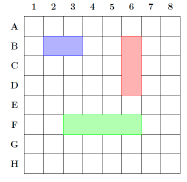
\includegraphics{Imagenes/batalla.png}
\end{figure}

\begin{itemize}
    \item[a)] Construya la función \texttt{actualizar\_flota(flota,posicion)} que retorne el diccionario flota actualizado, debido a un disparo realizado en la coordenada posición, la cual es entregada como tupla. En caso que el disparo no es certero, el diccionario permanece igual.
    \begin{lstlisting}[style=consola]
>>> actualizar_flota (flota1,('B',3))
>>> flota1
{'goleta': [('B',2)],'corbeta':[('F',3),('F',4),('F',5),
('F',6)],'fragata': [('B',6), ('C',6), ('D',6)]} 
    \end{lstlisting}
    \item[b)] Construya la función \texttt{estado\_actual(flota)} que retorne un diccionario con el estado actual de la flota, mostrando los porcentajes que queda de cada nave.
    \begin{lstlisting}[style=consola]
>>> flota1
{'goleta': [('B',2)],'corbeta':[('F',3),('F',4),('F',6)],
'fragata': [('B',6),('D',6)]}
>>> porcentajes = estado_actual(flota1)
>>> porcentajes
{'goleta':50,'corbeta':75,'fragata':66}
    \end{lstlisting}
\end{itemize}